\paragraph{VALL-E}

VALL-E is a language model developed by researchers at Microsoft for \ac{TTS} that treats \ac{TTS} as a conditional language modeling task~\cite{wang_neural_2023}. It generates text based on a given context, where the context in VALL-E is the acoustic tokens and phoneme prompts. VALL-E conditions on these inputs to produce the acoustic token sequence for speech synthesis.

VALL-E comprises two components: an audio codec that generates discrete acoustic tokens from speech waveforms and a neural language model that conditions these tokens and phoneme prompts to generate speech for unseen speakers in a zero-shot setting. The high-level architecture can be seen in Figure~\ref{fig:vall-e}.

\begin{figure}[ht]
    \centering
    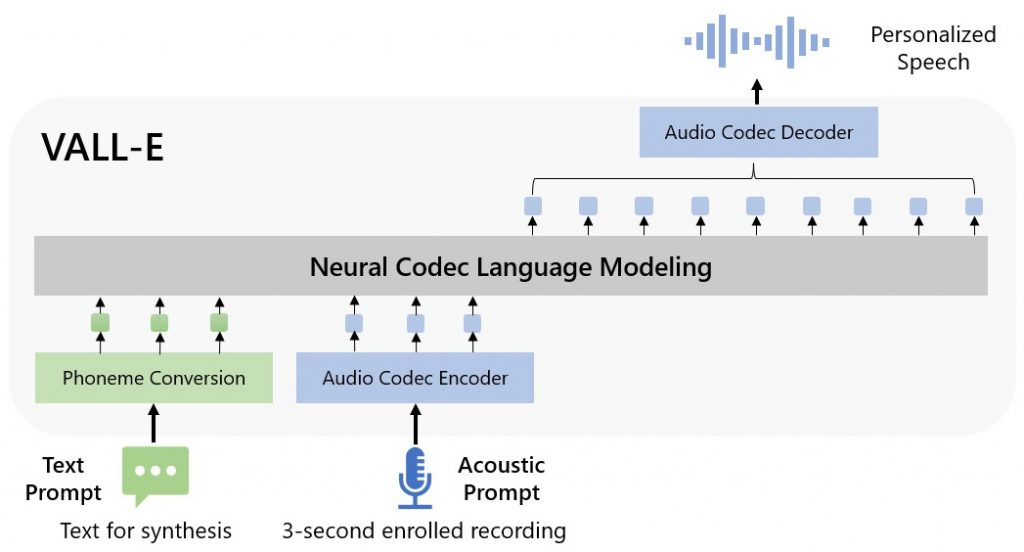
\includegraphics[width=\textwidth]{figures/2-sota/vall-e.jpg}
    \caption[VALL-E]{\textbf{VALL-E} --- The image was extracted from the source publication. It illustrates that both encodings derived from a linguistic prompt and an auditory prompt - provided via the codec encoder - are fed into a language model such as a transformer, and the resulting outputs are passed to the codec decoder to generate audio.}
    \label{fig:vall-e}
\end{figure}

The researchers trained VALL-E using the LibriLight dataset~\cite{kahn_libri-light_2020}, which consists of 60,000 hours of English speech from over 7,000 unique speakers. The proposed approach is robust to noise and generalizes well by leveraging a large and diverse dataset. Previous \ac{TTS} systems are typically trained with fewer data than VALL-E.

VALL-E's performance was evaluated on the LibriSpeech~\cite{panayotov_librispeech_2015} dataset, where all test speakers are unseen during training. VALL-E delivers high performance for speaker-adaptive \ac{TTS} in terms of speech naturalness and speaker similarity, as measured by comparative mean opinion score and similarity mean opinion score, respectively.

Qualitative analysis of VALL-E reveals several interesting findings. Firstly, VALL-E generates speech with diversity. As a result, the same input text can produce different speech outputs. This feature is important for downstream applications such as speech recognition, where diverse inputs with different speakers and acoustic environments are beneficial. The diversity of VALL-E makes it an ideal candidate for generating pseudo-data for speech recognition.

Another finding is that VALL-E maintains the acoustic environment of the prompt during speech synthesis. When the acoustic prompt has reverberation, VALL-E can synthesize speech with reverberation, whereas the baseline outputs clean speech. This can be attributed to VALL-E being trained on a large-scale dataset with diverse acoustic conditions, which allows it to learn acoustic consistency instead of only a clean environment during training.

Furthermore, VALL-E can preserve the emotion in the prompt during speech synthesis. The researchers selected acoustic prompts from the EmoV-DB dataset~\cite{adigwe_emotional_2018}, which contains speech with five emotions. VALL-E kept the exact emotion of the prompt in speech synthesis, even without fine-tuning on an emotional \ac{TTS} dataset.

VALL-E represents a significant advancement in \ac{TTS} technology, with its language model approach and use of audio codec codes as intermediate representations.

In summary, VALL-E is a language model-based \ac{TTS} system that utilizes audio codec codes as intermediate representations. It performs highly in speaker-adaptive \ac{TTS} and demonstrates exciting features such as speech diversity, acoustic environment consistency, and emotion preservation.